% This is part of Mes notes de mathématique
% Copyright (c) 2006-2015
%   Laurent Claessens, Carlotta Donadello
% See the file fdl-1.3.txt for copying conditions.

%+++++++++++++++++++++++++++++++++++++++++++++++++++++++++++++++++++++++++++++++++++++++++++++++++++++++++++++++++++++++++++
\section{Courbes de niveau}
%+++++++++++++++++++++++++++++++++++++++++++++++++++++++++++++++++++++++++++++++++++++++++++++++++++++++++++++++++++++++++++

Une technique utile pour se faire une idée de la forme d'une fonction en trois dimensions est de tracer les \defe{courbes de niveau}{courbe de niveau}. La courbe de niveau de hauteur $h$ est la courbe dans le plan donnée par l'équation
\begin{equation}
    f(x,y)=h.
\end{equation}

\begin{example}

    Dessinons par exemple les courbes de niveau de la fonction
    \begin{equation}
        f(x,y)=x+y+2.
    \end{equation}
    La courbe de niveau $h$ est donnée par l'équation $x+y+2=h$, c'est à dire
    \begin{equation}
        y(x)=-x+h-2.
    \end{equation}
    Par conséquent la courbe de niveau de hauteur $0$ est $y=-x-2$, celle de hauteur $5$ est $y=-x+3$, etc.
    
    Nous pouvons également nous aider de Sage pour ce faire :
    \begin{verbatim}
----------------------------------------------------------------------
| Sage Version 4.6.1, Release Date: 2011-01-11                       |
| Type notebook() for the GUI, and license() for information.        |
----------------------------------------------------------------------
sage: f(x,y)=x+y+2
sage: var('h')                   
h
sage: niveau(h,x)=solve(f(x,y)==h,y)[0].rhs()
sage: g1(x)=niveau(1,x)
sage: g1
x |--> -x - 1
    \end{verbatim}
    Ici la fonction \verb+g1+ est la courbe de niveau $1$. 

    Si on veut faire tracer une courbe de niveau, Sage peut le faire :
    \begin{verbatim}
        sage: implicit_plot(f(x,y)==1,(x,-3,3),(y,-4,4))
    \end{verbatim}
    Cela tracera la courbe de niveau $h=1$ dans la partie du plan $x\in\mathopen[ -3 , 3 \mathclose]$ et $y\in\mathopen[ -4,4 ,  \mathclose]$.
    
\end{example}

Il est bien entendu possible de créer automatiquement $50$ courbes de niveau et de demander de les tracer toutes sur le même graphe.
\VerbatimInput[tabsize=3]{courbeNiveau.py}

Le résultat est :

\begin{center}
    \ifpdf
        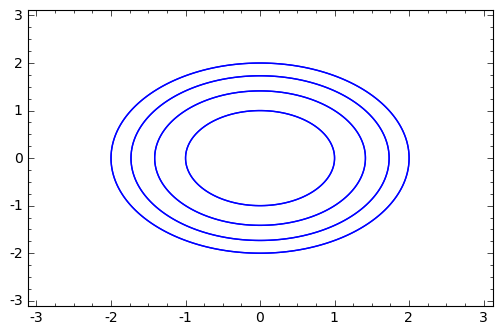
\includegraphics[width=8cm]{niveauCercles.png}
    \else
        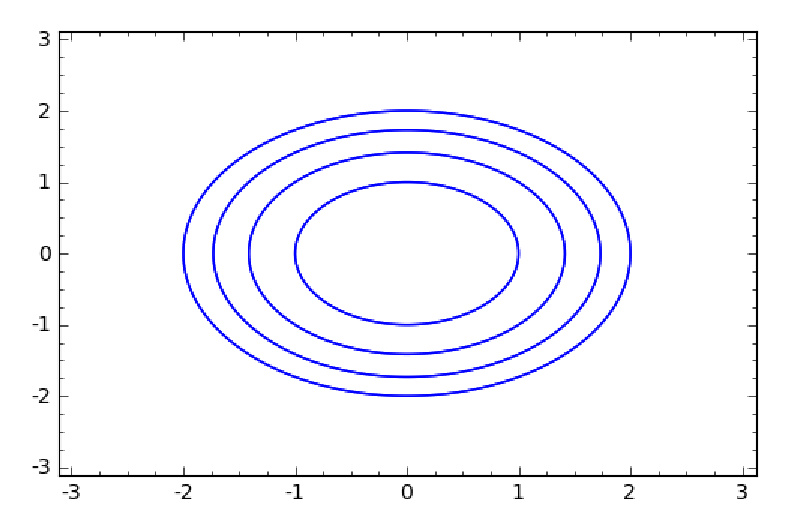
\includegraphics[width=8cm]{niveauCercles.eps}
    \fi
\end{center}
Notez que les courbes sont censées être des cercles : les axes $X$ et $Y$ n'ont pas la même échelle. Vous trouverez sur \href{http://uw.sagenb.org/home/pub/23/}{cette page} tout ce qu'il vous faudra pour créer des courbes de niveau avec Sage.

\begin{example}
    Un exemple plus riche en enseignements est celui de la fonction
    \begin{equation}
        f(x,y)=x^2-y^2.
    \end{equation}
    La courbe de niveau $h$ est donnée par l'équation $x^2-y^2=h$.

    Commençons par $h=0$. Dans ce cas nous avons $(x+y)(x-y)=0$ et par conséquent les courbes de niveau de hauteur zéro sont les deux droites $x+y=0$ et $x-y=0$.

    Voyons ensuite la courbe de niveau $h=1$. Cela est l'équation $x^2-y^2=1$, c'est à dire
    \begin{equation}
        y(x)=\pm\sqrt{x^2-1}.
    \end{equation}
    C'est une fonction qui n'est définie que pour $| x |\geq 1$. Avec $x=1$ nous avons $y=1$. Ensuite, lorsque $x$ grandit, $y$ grandit également, mais la courbe ne peut pas croiser la courbe de niveau $h=0$. Donc, suivant les notations de la figure \ref{LabelFigCQIXooBEDnfK}, la courbe de niveau «part» de $P$ et doit monter sans croiser les diagonales.

 % les figures CQIXooBEDnfK et KGQXooZFNVnW sont générées par le script MBFDooRFPyNW

%The result is on figure \ref{LabelFigCQIXooBEDnfK}. % From file CQIXooBEDnfK
\newcommand{\CaptionFigCQIXooBEDnfK}{La courbe de niveau $h=1$ de $x^2-y^2$. Notez qu'elle est en deux morceaux.}
\input{Fig_CQIXooBEDnfK.pstricks}

%The result is on figure \ref{LabelFigKGQXooZFNVnW}. % From file KGQXooZFNVnW
\newcommand{\CaptionFigKGQXooZFNVnW}{La courbe de niveau $x^2-y^2=-1$.}
\input{Fig_KGQXooZFNVnW.pstricks}

    En ce qui concerne la courbe de niveau $h=-1$, elle correspond à la courbe $y=\pm\sqrt{1+x^2}$ qui est définie pour tous les $x\in\eR$. Le même raisonnement que précédemment nous amène à la figure \ref{LabelFigKGQXooZFNVnW}.

\end{example}

Une autre façon de voir les courbe de niveau est de dire que la courbe de niveau de hauteur $h$ est la projection dans le plan $XY$ de la section du graphe de $f$ par le plan $z=h$.

On peut également définir le graphe de fonctions de trois (ou plus) variables. Le graphe de la fonction $f\colon D\subset\eR^3\to \eR$ est l'ensemble
\begin{equation}
    \big\{ \big( x,y,z,f(x,y,z) \big)\tq (x,y,z)\in D \big\}\subset \eR^4.
\end{equation}
De tels graphes ne peuvent pas être représentés sur une feuille de papier. Il est toutefois possible de définir les ensembles de niveaux :
\begin{equation}
    E_h=\big\{ (x,y,z)\in D\tq  f(x,y,z)=h\big\}.
\end{equation}
Ce sont des surfaces dans $\eR^3$ que l'on peut dessiner.

\begin{example}
    Les surfaces de niveau de la fonction $f(x,y,z)=x^2+y^2+z^2$ sont des sphères. Il n'y a pas de surfaces de niveau pour les «hauteurs» négatives.
\end{example}

\begin{example}
    Considérons la fonction $f(x,y,z)=x^2+y^2-z^2$. En coordonnées cylindrique, cette fonction s'écrit
    \begin{equation}
        f(r,\theta,z)=r^2-z^2.
    \end{equation}
    La surface de niveau $0$ est donnée par l'équation $r=| z |$. Cela fait un cercle à chaque hauteur, dont le rayon grandit linéairement avec la hauteur; le tout est donc un cône. C'est d'ailleurs le cône obtenu par rotation de la courbe de niveau $h=0$ que nous avions obtenue pour la fonction $x^2-y^2$.

    En ce qui concerne les ensembles de niveau positifs, ils sont donnés par
    \begin{equation}
        z=\pm\sqrt{x^2+y^2-h}.
    \end{equation}
    Notez qu'ils ne sont pas définis pour $r\geq h$. Cela pose un petit problème quand on veut le tracer à l'ordinateur :
    \begin{verbatim}
----------------------------------------------------------------------
| Sage Version 4.6.1, Release Date: 2011-01-11                       |
| Type notebook() for the GUI, and license() for information.        |
----------------------------------------------------------------------
sage: var('x,y')
(x, y)
sage: f(x,y)=sqrt(x**2+y**2-3)
sage: F=plot3d(f(x,y),(x,-5,5),(y,-5,5)) 
sage: G=plot3d(-f(x,y),(x,-5,5),(y,-5,5))    
sage: F+G
    \end{verbatim}
Le résultat est\footnote{Encore une fois : ça donne mieux à l'écran, et vous pouvez le faire bouger; je vous encourage à le faire !} :
    \begin{center}
        \ifpdf
            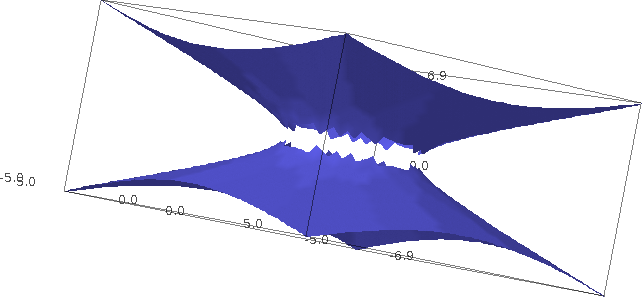
\includegraphics[width=15cm]{AdSmauvais.png}
        \else
            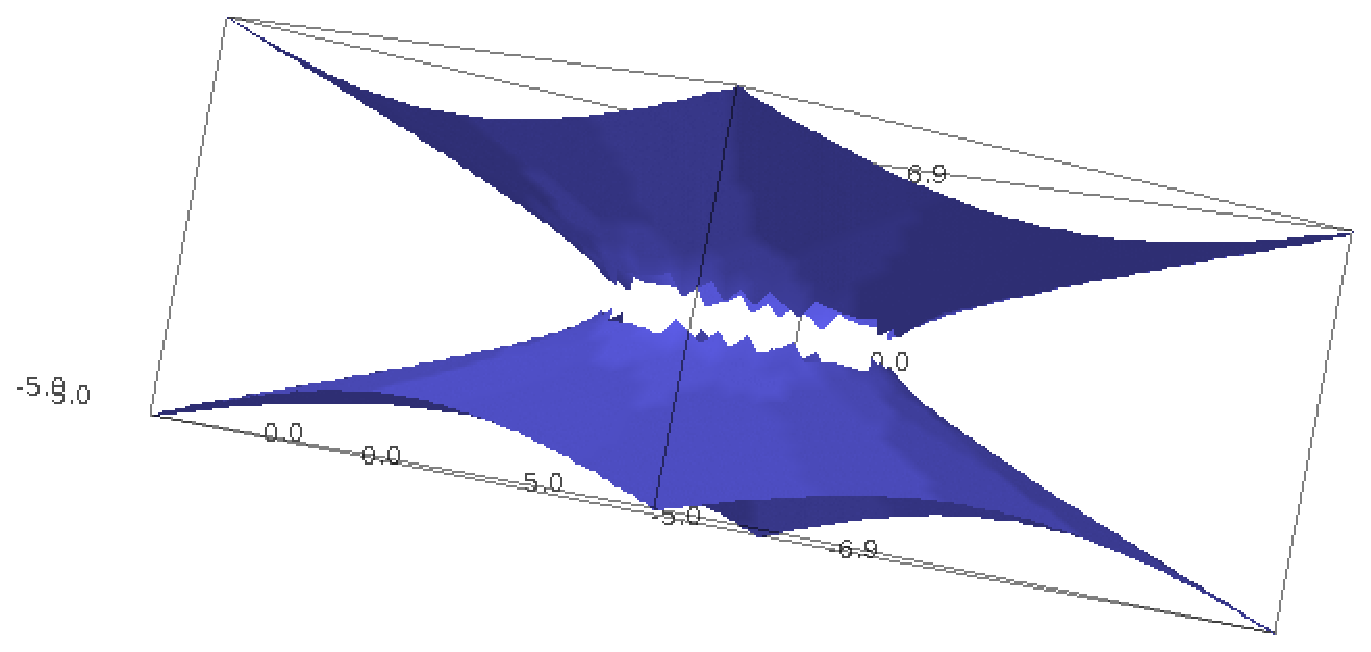
\includegraphics[width=15cm]{AdSmauvais.eps}
        \fi
    \end{center}
    On voit qu'il y a un grand trou au centre correspondant aux $z$ proches de zéro. Or d'après l'équation, il n'en est rien : en $z=0$ il y a bel et bien tout un cercle. Afin d'obtenir une meilleur image, il faut demander de tracer avec un maillage plus fin :
    \begin{verbatim}
----------------------------------------------------------------------
| Sage Version 4.6.1, Release Date: 2011-01-11                       |
| Type notebook() for the GUI, and license() for information.        |
----------------------------------------------------------------------
sage: var('x,y')
(x, y)
sage: f(x,y)=sqrt(x**2+y**2-3)
sage: F=plot3d(f(x,y),(x,-5,5),(y,-5,5),plot_points=300) 
sage: G=plot3d(-f(x,y),(x,-5,5),(y,-5,5),plot_points=300)
sage: F+G
    \end{verbatim}
    Le temps de calcul est un peu plus long, mais le résultat est meilleur :
    \begin{center}
        \ifpdf
            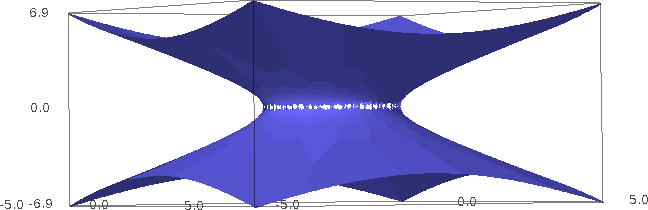
\includegraphics[width=15cm]{AdSbon.png}
        \else
            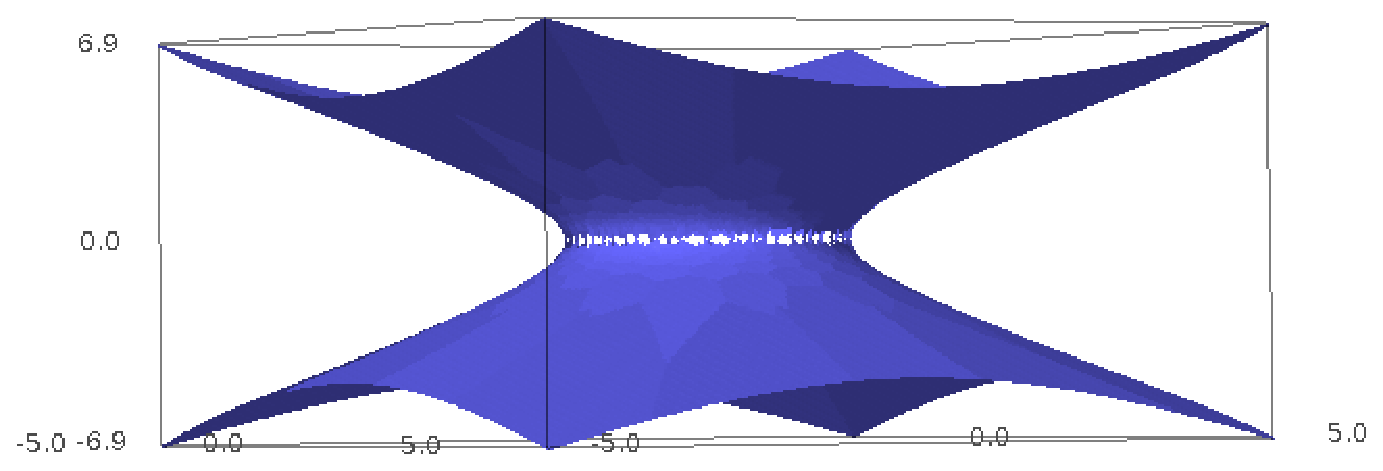
\includegraphics[width=15cm]{AdSbon.eps}
        \fi
    \end{center}
\end{example}

%+++++++++++++++++++++++++++++++++++++++++++++++++++++++++++++++++++++++++++++++++++++++++++++++++++++++++++++++++++++++++++
%\section{Calcul de limites}
%+++++++++++++++++++++++++++++++++++++++++++++++++++++++++++++++++++++++++++++++++++++++++++++++++++++++++++++++++++++++++++

%Incidemment, le lemme \ref{Def_diff2} nous donne une nouvelle technique pour calculer des limites à plusieurs variables, similaire à celle du développement asymptotique expliquée dans la section \ref{SecTaylorR}.

%En effet, la formule \eqref{def_diff2} nous permet d'écrire $f(x)$ sous la forme
%\begin{equation}
%	f(x)=f(a)+df(a).(x-a)+\sigma_f(a,x)\| x-a \|
%\end{equation}
%où la fonction $\sigma_f$ satisfait $\lim_{x\to a}\sigma_f(a,x)=0$. Ici, $x$ et $a$ sont des éléments de $\eR^m$.

%++++++++++++++++++++++++++++++++++++++++++++++++++++++++++++++++++++++++++++++++++++++++
\section{Fonctions de classe $\mathcal{C}^1$}
%++++++++++++++++++++++++++++++++++++++++++++++++++++++++++++++++++++++++++++++++++++++++++++++++++++++++++++++++++++++++++++++

Soit $f$ une fonction différentiable de $U$, ouvert de $\eR^m$, dans $\eR^n$. L'application différentielle de $f$ est une application  de $\eR^m$ dans $\mathcal{L}(\eR^m, \eR^n)$ 
\begin{equation}
  \begin{array}{rccc}
    df : & \eR^m & \to & \mathcal{L}(\eR^m, \eR^n)\\
& a& \mapsto & df_a.
  \end{array}
\end{equation}
Nous savons que $\mathcal{L}(\eR^m, \eR^n)$ est un espace vectoriel normé avec la définition \ref{DefDQRooVGbzSm}. Si $T$ est un élément dans $\mathcal{L}(\eR^m, \eR^n)$ alors la norme de $T$ est définie par 
\[
\|T\|_{\mathcal{L}(\eR^m, \eR^n)}=\sup_{x\in\eR^m} \frac{\|T(x)\|_n}{\|x\|_m}=\sup_{\begin{subarray}{l}
    x\in\eR^m\\
\|x\|_m\leq 1
  \end{subarray}} \|T(x)\|_n.
\]

Lorsqu'il existe un $M>0$ tel que $\| df(a) \|_{\aL(\eR^m,\eR^n)}<M$ pour tout $a$ dans $U$, nous disons que la différentielle de $f$ est \defe{bornée}{bornée!différentielle} sur $U$.

\begin{definition}
	La fonction $f$ est dite \defe{de classe $\mathcal{C}^1$}{fonction!de classe  $\mathcal{C}^1$} de $U\subset\eR^m$  dans $\eR^n$ si son application différentielle $df$ est continue de $\eR^m$ dans $\mathcal{L}(\eR^m, \eR^n)$. Nous écrivons $f\in\mathcal{C}^1(U,\eR^n)$\nomenclature{$\aC^1(U,\eR^n)$}{Les applications une fois continument dérivables}.
\end{definition}

\begin{proposition}		\label{PropDerContCun}
	Une fonction \( f\colon U\to \eR^n\) où \( U\) est ouvert dans \( \eR^m\) est de classe \( C^1\) si et seulement si les dérivées partielles de $f$ existent et sont continues.
\end{proposition}

\begin{proof}
	Supposons que les dérivées partielles de $f$ existent et sont continues. Nous savons alors déjà par la proposition \ref{Diff_totale} que la fonction $f$ est différentiable et qu'elle s'exprime sous la forme
	\[
		df_a(h)=\sum_{i=1}^{m}\partial_if (a)h_i, \qquad \forall a \in U,\,\forall h\in\eR^m.
	\]
	Pour montrer que $df$ est continue, nous devons montrer que la quantité $\| df(x)-df(a) \|_{\aL(\eR^m,\eR^n)}$ peut être rendue arbitrairement petite si $\| x-a \|_m$ est rendu petit. Nous avons
	\begin{equation}
		\begin{aligned}
			\| df_x-df_a \|_{\aL}&=\sup_{\| h \|=1}\| df_x(h)-df_a(h) \|\\
			&=\sup_{\| h \|_m=1}\left\|\sum_{i=1}^{m}\left(\partial_if (x)-\partial_if (a)\right)h_i\right\|_n\leq\\
			&\leq\sup_{\| h \|_m=1}\sum_{i=1}^{m} \left\|\left(\partial_if (x)-\partial_if (a)\right)\right\|_n|h_i|\leq\\
			&\leq\sup_{\| h \|_m=1} \|h\|_\infty\sum_{i=1}^{m} \left\|\left(\partial_if (x)-\partial_if (a)\right)\right\|_n\\
			&\leq \sum_{i=1}^m\| \partial_if(x)-\partial_if(a) \|.
		\end{aligned}
	\end{equation}
	Dans ce calcul, nous avons utilisé le fait que si $\| h \|_m\leq 1$, alors $\| h \|_{\infty}\leq 1$. Étant donné la continuité de $\partial_if$, la dernière ligne peut être rendue arbitrairement petite lorsque $x$ est proche e $a$.

Supposons maintenant que $f$ soit dans $\mathcal{C}^1(U,\eR^n)$. Alors 
\[
\left\|\partial_if (x)-\partial_if (a)\right\|_n= \left\|df(x).e_i-df(a).e_i\right\|_n \leq  \left\|df(x)-df(a)\right\|_{\mathcal{L}(\eR^m,\eR^n)},
\]  
la continuité de $df$ implique donc celle de $\partial_i f$ pour tout $i$ dans $\{1,\ldots,m\}$.
\end{proof}
\begin{proposition}
  Soient $U$ un ouvert de $\eR^m$ et $V$ un ouvert de $\eR^n$. Soient $f: U\to V$  dans $\mathcal{C}^1(U,V)$ et $g: V \to \eR^p$ dans $\mathcal{C}^1(V,\eR^n)$.  Alors la fonction composée $g\circ f: U\to \eR^p $ est dans $\mathcal{C}^1(U,\eR^p)$.
\end{proposition}
\begin{proof} On fixe $a$ dans $U$ 
  \begin{equation}
    \begin{aligned}
     \big\|d(g\circ f)(x)&-d(g\circ f)(a)\big\|_{\mathcal{L}(\eR^m,\eR^p)}\\
     &=\left\|dg(f(x))\circ df(x)-dg(f(a))\circ df(a)\right\|_{\mathcal{L}(\eR^m,\eR^p)}\leq\\
&\leq \left\|\left(dg(f(x))-dg(f(a))\right)\circ df(x)\right\|_{\mathcal{L}(\eR^m,\eR^p)}+\\
&\quad+ \left\|dg(f(a))\circ \left(df(x)-df(a)\right)\right\|_{\mathcal{L}(\eR^m,\eR^p)}\leq\\
&\leq \left\|dg(f(x))-dg(f(a))\right\|_{\mathcal{L}(\eR^n,\eR^p)}\left\| df(x)\right\|_{\mathcal{L}(\eR^m,\eR^n)}+\\
&\quad+ \left\|dg(f(a))\right\|_{\mathcal{L}(\eR^n,\eR^p)}\left\| df(x)-df(a)\right\|_{\mathcal{L}(\eR^n,\eR^p)}.\\
    \end{aligned}
  \end{equation}
On peut conclure en passant à la limite $x\to a$ parce que les fonctions $f$, $g$, $df$ et $dg$ sont continues, de telle sorte que
\begin{equation}
	\begin{aligned}[]
		\lim_{x\to a} dg\big( f(x) \big)=dg\big( f(a) \big)\\
		\lim_{x\to a} df(x)=df(a).
	\end{aligned}
\end{equation}
\end{proof}

\begin{remark}
  On peut prouver le même résultat en utilisant la continuité de l'application bilinéaire 
\begin{equation}
  \begin{array}{rccc}
    \circ : & \mathcal{C}^1(U,V)\times\mathcal{C}^1(V,\eR^p)  & \to & \mathcal{L}(U, \eR^p)\\
& (T,S)& \mapsto & T\circ S.
  \end{array}
\end{equation}
\end{remark}
